\documentclass[11pt,aspectratio=169]{beamer}
\usepackage[italian]{babel}
\usepackage[latin1]{inputenc}
\usepackage{graphicx}
\usepackage{listings}
\usepackage[export]{adjustbox}
% Custom bullets
\usepackage{pifont}
\usepackage[useregional]{datetime2}
\usepackage{tikz}
\usepackage[table]{colortbl}
\usepackage{venndiagram}
\usepackage{amsmath}
\usetikzlibrary{shapes.geometric}
\usetikzlibrary{decorations.markings}
\usetikzlibrary{calc}
\usetikzlibrary{positioning}
\usetikzlibrary{positioning, arrows.meta}

% custom legend
\newcommand{\cbox}[1]{\raisebox{\depth}{\fcolorbox{black}{#1}{\null}}}

\usetheme{Madrid}
\usecolortheme{spruce}

% Redefine labels
\deftranslation[to=Italian]{Section}{Sezione}
\deftranslation[to=Italian]{Subsection}{Sottosezione}


\author[Gianluca Lanchini \and Piermichele Rosati]{Gianluca Lanchini \and Piermichele Rosati}

\institute[]{\large Universit\`a di Camerino\\ \footnotesize Tutorato - Basi di Dati}

\title[Normalizzazione dei Dati]{10. Normalizzazione dei Dati}
\subtitle{Ridondanza, Forme normali}
\setbeamertemplate{navigation symbols}{}
\setbeamertemplate{section in toc}[sections numbered]
\setbeamertemplate{subsection in toc}[subsections numbered]
%\titlegraphic{
\includegraphics[width=6cm]{img/unicam-logo.jpg}}
\makeatletter
\setbeamertemplate{footline}{
    \leavevmode%
    \hbox{%
        \begin{beamercolorbox}[wd=.333333\paperwidth,ht=2.25ex,dp=1ex,center]{author in head/foot}%
            \usebeamerfont{author in head/foot}\insertshortauthor
        \end{beamercolorbox}%
        \begin{beamercolorbox}[wd=.333333\paperwidth,ht=2.25ex,dp=1ex,center]{title in head/foot}%
            \usebeamerfont{title in head/foot}\insertshorttitle
        \end{beamercolorbox}%
        \begin{beamercolorbox}[wd=.333333\paperwidth,ht=2.25ex,dp=1ex,right]{date in head/foot}%
            \usebeamerfont{date in head/foot}\today\hspace*{5 em}
            \insertframenumber{} / \inserttotalframenumber\hspace*{2ex} 
        \end{beamercolorbox}%
    }%
    \vskip0pt%
}
\makeatother


\AtBeginSection[]
{
\begin{frame}<beamer>
\frametitle{Indice}
\tableofcontents[currentsection]
\end{frame}
}

\begin{document}
\begin{frame}
\centering

\includegraphics[width=5.5cm]{../img/unicam-logo.jpg}
\date{\today}
\titlepage
\end{frame}
\addtobeamertemplate{frametitle}{}{%
\begin{tikzpicture}[remember picture,overlay]
\node[anchor=north east,yshift=2pt] at (current page.north east) {
\includegraphics[height=2cm]{../img/unicam-logo-notext.png}};
\end{tikzpicture}}

%\begin{frame}
%\titlepage
%\end{frame}

\section{La Normalizzazione delle Relazioni}
\def\InventarioModified{
    \textbf{Inventario}
    
    \begin{tabular}{|c|c|c|c|c|}
        \hline
        \rowcolor{cyan!30}Numero & Prodotto & Magazzino & Quantita & IndirizzoMagazzino \\
        \hline
        1 & 545 & CA1 & 800 & Via Tonale, 12 \\ \hline
        2 &545 & PA2 & 700 & Via Mazzini, 25 \\ \hline
        3 & 545 & VE1 & 356 & Calle Corta, 5 \\ \hline
        4 & 100 & CA1 & 245 & Via Tonale, 12 \\ \hline
        5 & 200 & VE1 & 230 & Calle Corta, 5 \\ \hline
        6 & 545 & PA1 & 370 & Via Garibaldi, 38 \\ \hline
        7 & 100 & PA2 & 350 & Via Mazzini, 25 \\ \hline
        8 & 100 & VE1 & 720 & Calle Corta, 5 \\ \hline
    \end{tabular}
}
\def\InventarioModifiedPK{
    \textbf{Inventario}
    
    \begin{tabular}{|c|c|c|c|}
        \hline
        \rowcolor{cyan!30} \underline{Prodotto} & \underline{Magazzino} & Quantita & IndirizzoMagazzino \\
        \hline
        545 & CA1 & 800 & Via Tonale, 12 \\ \hline
        545 & PA2 & 700 & Via Mazzini, 25 \\ \hline
        545 & VE1 & 356 & Calle Corta, 5 \\ \hline
        100 & CA1 & 245 & Via Tonale, 12 \\ \hline
        200 & VE1 & 230 & Calle Corta, 5 \\ \hline
        545 & PA1 & 370 & Via Garibaldi, 38 \\ \hline
        100 & PA2 & 350 & Via Mazzini, 25 \\ \hline
        100 & VE1 & 720 & Calle Corta, 5 \\ \hline
    \end{tabular}
}
\def\InventarioNegozi{
    \begin{minipage}[t]{0.48\linewidth}
        \begin{center}
            \textbf{Inventario}
            
            \begin{tabular}{|c|c|c|}
            \hline
            \rowcolor{cyan!30} \underline{Prodotto} & \underline{Magazzino} & Quantita \\
            \hline
            545 & CA1 & 800 \\ \hline
            545 & PA2 & 700 \\ \hline
            545 & VE1 & 356 \\ \hline
            100 & CA1 & 245 \\ \hline
            200 & VE1 & 230 \\ \hline
            545 & PA1 & 370 \\ \hline
            100 & PA2 & 350 \\ \hline
            100 & VE1 & 720 \\ \hline
        \end{tabular}
        \end{center}
    \end{minipage}%
    \hfill%
    \begin{minipage}[t]{0.5\linewidth}
        \begin{center}
            \textbf{Negozi}
    
            \begin{tabular}{|c|c|}
            \hline
            \rowcolor{cyan!30} \underline{Magazzino} & IndirizzoMagazzino \\
            \hline
            CA1 & Via Tonale, 12 \\ \hline
            PA1 & Via Garibaldi, 38 \\ \hline
            PA2 & Via Mazzini, 25 \\ \hline
            VE1 & Calle Corta, 5 \\ \hline
        \end{tabular}
        \end{center}
    \end{minipage}
}
\begin{frame}{La Ridondanza dei Dati}
\begin{minipage}{0.9\textwidth}
    \begin{block}{Ridondanza}
        La \textbf{ridondanza} dei dati si verifica quando le stesse informazioni sono memorizzate in pi\`u di un posto.
    \end{block}
\end{minipage}
\pause
    \begin{block}{Incongruenza}
        La ridondanza porta a problemi non indifferenti come \textbf{incongruenza}: quando aggiorniamo i dati ridondanti, questi potrebbero venire aggiornati in alcune tabelle mentre in altre no.
    \end{block}
\pause
    \begin{block}{Inconsistenza}
        L'incongruenza porta spesso a \textbf{inconsistenza}: quando abbiamo a disposizione dati ridondanti, potremmo non essere pi\`u in grado di capire quali tra questi dati sono affidabili, perch\`e non si sa quale sia il dato corretto.
    \end{block}
\end{frame}
%
\begin{frame}{La Ridondanza dei Dati}
\begin{minipage}[t]{0.55\linewidth}
    \begin{center}
        \textbf{Inventario}
        
        \begin{tabular}{|c|c|c|c|}
            \hline
            \rowcolor{cyan!30}Prodotto & Magazzino & Quantita & IndirizzoMagazzino \\
            \hline
            545 & CA1 & 800 & Via Tonale, 12 \\ \hline
            545 & PA2 & 700 & Via Mazzini, 25 \\ \hline
            545 & VE1 & 356 & Calle Corta, 5 \\ \hline
            100 & CA1 & 245 & Via Tonale, 12 \\ \hline
            200 & VE1 & 230 & Calle Corta, 5 \\ \hline
            545 & PA1 & 370 & Via Garibaldi, 38 \\ \hline
            100 & PA2 & 350 & Via Mazzini, 25 \\ \hline
            100 & VE1 & 720 & Calle Corta, 5 \\ \hline
        \end{tabular}
    \end{center}
\end{minipage}%
\hfill%
\begin{minipage}[t]{0.35\linewidth}
    \textbf{Inventario} \`e una tabella ben organizzata?
    \pause
    \newline
    \\Ovviamente no!
    
    L'indirizzo di un certo magazzino \`e ripetuto ogni volta che quel magazzino \`e referenziato tramite il codice e, pertanto, i dati nel campo IndirizzoMagazzino sono ridondanti.
\end{minipage}
    
\end{frame}
%
\begin{frame}{La Ridondanza dei Dati}
La ridondanza va evitata, non solo perch\`e viene sprecato spazio su disco ma, sopratutto per le possibili \textbf{anomalie} che si possono presentare nel corso delle diverse fasi del trattamento dei dati:
\pause
\begin{itemize}[<+->]
    \item \textbf{anomalia di aggiornamento}: se il magazzino CA1 cambia indirizzo bisogna modificare il valore di IndirizzoMagazzino in tutte le occorrenze di CA1 di \textbf{Inventario}; se per qualunque ragione, l' aggiornamento avviene solo in alcune delle righe interessate, i dati memorizzati diventano inconsistenti.
    \item \textbf{anomalia di cancellazione}: se un magazzino si svuota vengono perse le informazioni sul suo indirizzo;
    \item \textbf{anomalia di inserimento}: quando viene aperto un nuovo magazzino, in mancanza di merci a magazzino, mancano le informazioni sul suo indirizzo.
\end{itemize}
\end{frame}
%
\begin{frame}{La Ridondanza dei Dati}
Per evitare ridonanza di IndirizzoMagazzino possiamo pensare di sostituire alla tabella \textbf{Inventario} la seguente coppia di tabelle:
\pause
\vspace{.2cm}

\InventarioNegozi
\end{frame}
%
\begin{frame}{La Ridondanza dei Dati}
La scomposizione nelle 2 tabelle non causa perdita di informazione, in quanto la tabella di partenza potr\`a essere ricostruita mediante congiunzione tra \textbf{Inventario} e \textbf{Negozi} sul campo Magazzino.
\pause

Le tabelle avranno il seguente schema:

\pause
\textbf{Inventario}(\underline{Prodotto}, \underline{Magazzino}$^*$, Quantita)\\
\pause

\textbf{Negozi}(\underline{Magazzino}$^*$, IndirizzoMagazzino)
\end{frame}
%
\begin{frame}{La Ridondanza dei Dati}
\begin{itemize}[<+->]
    \item Sono stati definiti opportuni criteri che dono essere soddisfatti dalle relazioni per evitare la \textbf{ridonanza} dei dati e le possibili anomalie che ne conseguono;
    \item Tali criteri definiscono le caratteristiche che devono essere soddisfatte da una relazione ben strutturata e prendono il nome di \textbf{forme normali};
    \item Le forme normali sono di livello crescente , e sono accompagnate da algoritmi per la trasformazione di una tabella, che viola una forma normale, in un insieme di tabelle che rispettano il criterio;
    \item Tale processo di trasformazione prende il nome di \textbf{normalizzazione}.
\end{itemize}
\end{frame}
%
\begin{frame}{Normalizzazione}
\vspace{-1.5cm}
Regole e procedimenti volti ad eliminare (o almeno a ridurre) le \textbf{ridondanze} in un database e ad evitare situazioni di \textbf{incoerenza}.
\vspace{2em}

\uncover<2->{Esistono vari livelli di normalizzazione, chiamati forme normali, \\che indicano la qualit\`a dello schema del database.}

\begin{tikzpicture}[remember picture, overlay]
    \node[anchor=south east, xshift=-0.5cm, yshift=-0.8cm] at (current page.south east) {
        
\includegraphics[width=0.3\textwidth]{img/goku1.png}
    };
\end{tikzpicture}

\end{frame}
%
\begin{frame}{Forme Normali}
\vspace{-.8cm}
\begin{center}
    \begin{tikzpicture}
    
        % Draw rectangles with rounded corners and place text above the inner content
        \node[draw, rounded corners, minimum width=8cm, minimum height=0.8cm, fill=white] (outer) {
            \begin{tikzpicture}
                \node[draw, rounded corners, minimum width=7.5cm, minimum height=0.9cm, fill=white] (second) {
                    \begin{tikzpicture}
                        \node[draw, rounded corners, minimum width=7cm, minimum height=0.8cm, fill=white] (third) {
                            \begin{tikzpicture}
                                \node[draw, rounded corners, minimum width=6.5cm, minimum height=0.7cm, fill=white] (fourth) {
                                    \begin{tikzpicture}
                                        \node[draw, rounded corners, minimum width=6cm, minimum height=1cm, fill=white] (fifth) {
                                            \begin{tikzpicture}
                                                \node[draw, rounded corners, minimum width=5.5cm, minimum height=0.5cm, fill=white] (inner) {5NF};
                                            \end{tikzpicture}
                                        };
                                        \node[above=of inner] {4NF};
                                    \end{tikzpicture}
                                };
                                \node[above=of fifth] {BCNF};
                            \end{tikzpicture}
                        };
                        \node[above=of fourth] {3NF};
                    \end{tikzpicture}
                };
                \node[above=of third] {2NF};
            \end{tikzpicture}
        };
        \node[above=of second] {1NF};
    
    \end{tikzpicture}
    \end{center}
% \begin{figure}[h]
%     \centering 
%     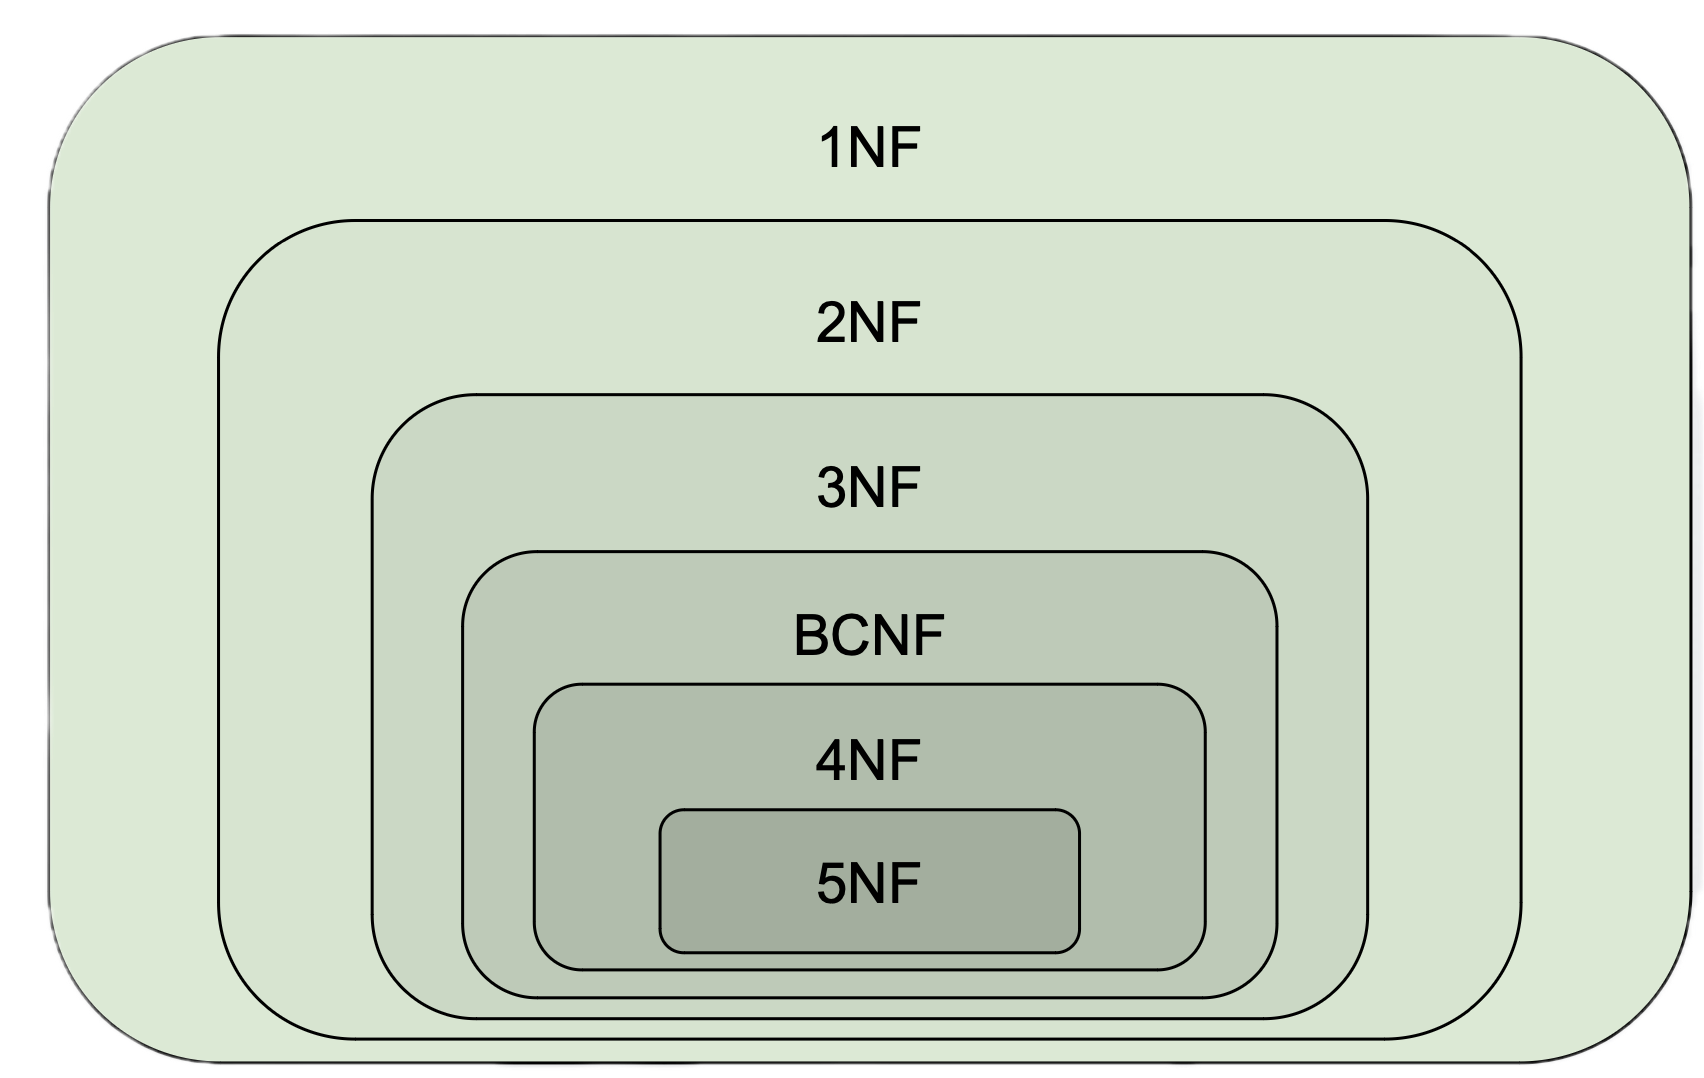
\includegraphics[width=0.7\textwidth]{img/normalizzazione.png} 
% \end{figure}
\end{frame}
%
\begin{frame}{Concetti Base}
    \begin{itemize}[<+->]
        \item \textbf{Superchiave:} \`e un attributo o un insieme di attributi che identificano univocamente una tupla in una tabella.
        \item \textbf{Chiave candidata} \`e una superchiave minimale, ovvero nessun sottoinsieme di attributi pu\`o essere considerato una superchiave della tabella;
        \item \textbf{Chiave o chiave primaria} \`e la chiave candidata selezionata per identificare in modo univoco una tupla della tabella (ci possono essere molte chiavi candidate ma una sola chiave primaria);
        \item \textbf{Chiave alternativa} \`e una qualsiasi chiave candidata che non \`e stata scelta come chiave primaria;
        \item \textbf{Attributo non-chiave} o \textbf{non primo} \`e un attributo che non fa parte della chiave. In caso contrario viene chiamato \textbf{attributo chiave} o \textbf{primo}.
    \end{itemize}
\end{frame}
%
\begin{frame}{Esempio: Inventario}
\vspace{-1cm}
\begin{center}
    \InventarioModified
\end{center}
\pause
\textbf{Superchiavi}:
\pause
\begin{itemize}[<+->]
    \item \{Numero\}
    \item \{Numero, Prodotto\}
    \item \{Numero, Prodotto, Magazzino\}
    \item \{Numero, Prodotto, Magazzino, Quantita\}
    \item \ldots
\end{itemize}
\begin{tikzpicture}[remember picture, overlay]
    \node[anchor=south east, xshift=0.3cm, yshift=-0.5cm] at (current page.south east) {
        
\includegraphics[width=0.3\textwidth]{img/goku_piccolo.png}
    };
\end{tikzpicture}
\end{frame}
%
\begin{frame}{Esempio: Inventario}
\vspace{-1cm}
\begin{center}
    \InventarioModified
\end{center}
\pause
\textbf{Chiavi candidate}:
\pause
\begin{itemize}[<+->]
    \item \{Numero\} \ding{51}
    \item \{Prodotto, Magazzino\} \ding{51}
    \item \{Prodotto, Magazzino, Quantita\} \ding{55}
    \pause 
    
    {\small NO! perch\`e contiene il sottoinsieme \{Prodotto, Magazzino\}\\ che \`e una chiave candidata.}
\end{itemize}
\begin{tikzpicture}[remember picture, overlay]
    \node[anchor=south east, xshift=0.3cm, yshift=-0.5cm] at (current page.south east) {
        
\includegraphics[width=0.3\textwidth]{img/goku_piccolo.png}
    };
\end{tikzpicture}
\end{frame}
%
\begin{frame}{Esempio: Inventario}
\vspace{-1cm}
\begin{center}
    \InventarioModified
\end{center}
\pause
\textbf{Attributi non-chiave}:
\pause
\begin{itemize}[<+->]
    \item \{Quantita\}
    \item \{IndirizzoMagazzino\}
\end{itemize}
\begin{tikzpicture}[remember picture, overlay]
    \node[anchor=south east, xshift=0.3cm, yshift=-0.5cm] at (current page.south east) {
        
\includegraphics[width=0.3\textwidth]{img/goku_piccolo.png}
    };
\end{tikzpicture}
\end{frame}
%
\begin{frame}{Esempio: Inventario}
\vspace{-1cm}
\begin{center}
    \InventarioModified
\end{center}
\pause
\textbf{Chiave primaria}:
Se il progettista sceglie Numero come \textbf{chiave primaria};

\textbf{Chiavi alternative}:
\pause
\begin{itemize}[<+->]
    \item \{Prodotto, Magazzino\}
\end{itemize}
\begin{tikzpicture}[remember picture, overlay]
    \node[anchor=south east, xshift=0.3cm, yshift=-0.5cm] at (current page.south east) {
        
\includegraphics[width=0.3\textwidth]{img/goku_piccolo.png}
    };
\end{tikzpicture}
\end{frame}
%
\begin{frame}{Concetti Base}
    \begin{table}[h]
    \centering
    \begin{tabular}{|c|c|c|c|c|}
        \hline
        \rowcolor{cyan!30} \textbf{\underline{Nome}} & \textbf{Razza} & \textbf{\underline{AnnoNascita}} & \textbf{Altezza(cm)} & \textbf{Peso(kg)} \\ \hline
        Goku & Saiyan & 737 & 175 & 62 \\ \hline
        Gohan & Saiyan & 757 & 176 & 61 \\ \hline
        Vegeta & Saiyan & 732 & 164 & 56 \\ \hline
        Gohan & Umano & 658 & 158 & 50 \\ \hline
        Piccolo & Namecciano & 753 & 226 & 116 \\ \hline
    \end{tabular}
\end{table}
\uncover<2->{
\textbf{Superchiavi}:
\\\{Nome, Razza, AnnoNascita, Altezza, Peso\}
\\\{Nome, Razza\}\only<3> {\hspace{0.5cm}\textcolor{red}{chiave candidata}}
\\\{Nome, AnnoNascita\}\only<3> {\hspace{0.5cm}\textcolor{red}{chiave candidata}} \only<4>{\hspace{0.5cm}\textcolor{red}{chiave primaria}}
\\\{Nome, Razza, AnnoNascita\}
etc \ldots}
\begin{tikzpicture}[remember picture, overlay]
    \node[anchor=south east, xshift=0.3cm, yshift=-0.5cm] at (current page.south east) {
        
\includegraphics[width=0.3\textwidth]{img/goku_piccolo.png}
    };
\end{tikzpicture}

\end{frame}
%
\begin{frame}{Concetti Base}
\begin{table}[h]
    \centering
    \begin{tabular}{|c|c|c|c|c|}
        \hline
        \rowcolor{cyan!30} \textbf{\underline{Nome}} & \textbf{Razza} & \textbf{\underline{AnnoNascita}} & \textbf{Altezza(cm)} & \textbf{Peso(kg)} \\ \hline
        Goku & Saiyan & 737 & 175 & 62 \\ \hline
        Gohan & Saiyan & 757 & 176 & 61 \\ \hline
        Vegeta & Saiyan & 732 & 164 & 56 \\ \hline
        Gohan & Umano & 658 & 158 & 50 \\ \hline
        Piccolo & Namecciano & 753 & 226 & 116 \\ \hline
    \end{tabular}
\end{table}
\vspace{0.2cm}

\textbf{Primo}: \{Nome, Razza\}\\
\textbf{Non-primo}: \{Altezza, Peso\}
\begin{tikzpicture}[remember picture, overlay]
    \node[anchor=south east, xshift=0.3cm, yshift=-0.5cm] at (current page.south east) {
        
\includegraphics[width=0.3\textwidth]{img/goku_piccolo.png}
    };
\end{tikzpicture}
\end{frame}
%
\begin{frame}{La Dipendenza Funzionale}
\begin{minipage}{0.9\textwidth}
\begin{block}{Dipendenza funzionale}
    Si ha \textbf{dipendenza funzionale} tra attributi quando il valore di un insieme di attributi A determina un singolo valore dell'attributo B e si indica con: A $ \rightarrow $ B.

    Si dice anche che B dipende funzionalmente da A, o che A \`e un \textbf{determinante} per B e si indica con A $ \rightarrow $ B.
\end{block}
\end{minipage}
\pause
\begin{itemize}[<+->]
    \item A $ \rightarrow $ B si legge ``A determina B'' oppure ``B dipende funzionalmente da A'';
    \item Se B non \`e contenuto nell`insieme A allora la dipendenza viene detta \textbf{non banale}.
    
    In caso contrario viene detta \textbf{banale}.
\end{itemize}
\pause
\begin{block}{Nota bene}
    Ogni chiave candidata di una relazione \`e un determinante per tutti i suoi attributi e, viceversa, ogni determinante per tutti gli attributi di una relazione \`e chiave candidata per quella relazione.
\end{block}
\end{frame}
%
\begin{frame}{La Dipendenza Funzionale: Esempio Inventario}
\vspace{-0.7cm}
\InventarioModified

Notiamo che:
\begin{itemize}[<+->]
    \item da Numero = 4: 4 $ \rightarrow $ (100, CA1, 245, `Via Tonale, 12');
    \item da \{Prodotto, Magazzino\} = \{545, PA2\}:
    
    \{545, PA2\} $ \rightarrow $ (2, 700, `Via Mazzini, 25');
    \item da Magazzino = VE1: VE1 $ \rightarrow $ `Calle Corta, 5'.
\end{itemize}
\begin{tikzpicture}[remember picture, overlay]
    \node[anchor=south east, xshift=0.3cm, yshift=-0.5cm] at (current page.south east) {
        
\includegraphics[width=0.3\textwidth]{img/goku_piccolo.png}
    };
\end{tikzpicture}   
\end{frame}
%
\begin{frame}{La Dipendenza Funzionale: Esempio Inventario}
\vspace{-0.7cm}
\InventarioModified
\vspace{.2cm}

Generalizzando si intuisce che:
\begin{itemize}[<+->]
    \item Numero \`e determinante per ogni attributo di \textbf{Inventario};
    \item \{Prodotto, Magazzino\} \`e determinante per ogni attributo di\\ \textbf{Inventario};
    \item Magazzino \`e determinante per IndirizzoMagazzino.
\end{itemize}
\begin{tikzpicture}[remember picture, overlay]
    \node[anchor=south east, xshift=0.3cm, yshift=-0.5cm] at (current page.south east) {
        
\includegraphics[width=0.3\textwidth]{img/goku_piccolo.png}
    };
\end{tikzpicture}   
\end{frame}
%
\begin{frame}{La Dipendenza Funzionale: Esempio Inventario}
\vspace{-0.7cm}
\InventarioModified
\vspace{.2cm}

In simboli:
\begin{itemize}[<+->]
    \item Numero $ \rightarrow $ (Prodotto, Magazzino, Quantita, IndirizzoMagazzino);
    \item {\small \{Prodotto, Magazzino\} $ \rightarrow $ (Numero, Quantita, IndirizzoMagazzino);}
    \item Magazzino $ \rightarrow $ IndirizzoMagazzino.
\end{itemize}
\begin{tikzpicture}[remember picture, overlay]
    \node[anchor=south east, xshift=0.3cm, yshift=-0.5cm] at (current page.south east) {
        
\includegraphics[width=0.3\textwidth]{img/goku_piccolo.png}
    };
\end{tikzpicture}   
\end{frame}
%
\begin{frame}{La Dipendenza Funzionale: Esempio Dragon Ball}
\begin{table}[h]
    \centering
    \begin{tabular}{|c|c|c|c|c|}
        \hline
        \rowcolor{cyan!30} \textbf{\underline{NOME}} & \textbf{RAZZA} & \textbf{\underline{ANNO NASCITA}} & \textbf{ALTEZZA (cm)} & \textbf{PESO (kg)} \\ \hline
        Goku & Saiyan & 737 & 175 & 62 \\ \hline
        Gohan & Saiyan & 757 & 176 & 61 \\ \hline
        Vegeta & Saiyan & 732 & 164 & 56 \\ \hline
        Gohan & Umano & 658 & 158 & 50 \\ \hline
        Piccolo & Namecciano & 753 & 226 & 116 \\ \hline
    \end{tabular}
\end{table}
\pause
\textbf{Dipendenze funzionali}:
\pause
\begin{itemize}[<+->]
    \item \{NOME, ANNO NASCITA\} $ \rightarrow $ RAZZA
    \item \{NOME, ANNO NASCITA\} $ \rightarrow $ ALTEZZA
    \item \{NOME, ANNO NASCITA\} $ \rightarrow $ PESO
    \item \{NOME, ANNO NASCITA\} $ \rightarrow $ NOME 
    
    \textcolor{red}{dipendenza funzionale banale}
\end{itemize}
\begin{tikzpicture}[remember picture, overlay]
    \node[anchor=south east, xshift=0.3cm, yshift=-0.5cm] at (current page.south east) {
        
\includegraphics[width=0.3\textwidth]{img/goku_piccolo.png}
    };
\end{tikzpicture}   
\end{frame}
%
\begin{frame}{La Dipendenza Funzionale: Esempio Dragon Ball}
    
\begin{table}[h]
    \centering
    \begin{tabular}{|c|c|c|c|}
        \hline
        \rowcolor{cyan!30} \textbf{\underline{ID}} & \textbf{NOME} & \textbf{TRASFORMAZIONE} & \textbf{CAPELLI} \\ \hline
        0 & Goku & Normale & Neri \\ \hline
        1 & Goku & Super Saiyan & Biondi \\ \hline
        2 & Goku & Super Saiyan 2 & Biondi \\ \hline
        3 & Goku & Super Saiyan 3 & Biondi \\ \hline
        4 & Vegeta & Normale & Neri \\ \hline
    \end{tabular}
\end{table}
\pause
\textbf{Dipendenze funzionali}:
\pause
\begin{itemize}[<+->]
    \item \{ID\} $ \rightarrow $ NOME
    \item \{ID\} $ \rightarrow $ TRASFORMAZIONE
    \item \{ID\} $ \rightarrow $ CAPELLI
    \item \{TRASFORMAZIONE\} $ \rightarrow $ CAPELLI
\end{itemize}
\begin{tikzpicture}[remember picture, overlay]
    \node[anchor=south east, xshift=0.3cm, yshift=-0.5cm] at (current page.south east) {
        
\includegraphics[width=0.3\textwidth]{img/goku_piccolo.png}
    };
\end{tikzpicture}
\end{frame}
%
\begin{frame}{La Dipendenza Transitiva}
    \begin{block}{Dipendenza Transitiva}
        Si ha \textbf{dipendenza transitiva} tra attributi quando un attributo A determina B e B determina C; si dice allora che C dipende transitivamente da A: se A $ \rightarrow $ B e B $ \rightarrow $ C allora A $ \rightarrow $ C transitivamente.
    \end{block}
Un esempio di dipendenza transitiva nella tabella Inventario:
    \begin{itemize}[<+->]
        \item Numero $ \rightarrow $ Magazzino e Magazzino $ \rightarrow $ IndirizzoMagazzino.
        \item Numero $ \rightarrow $ IndirizzoMagazzino transitivamente.
    \end{itemize}
\end{frame}
%
\begin{frame}{Prima Forma Normale (1NF)}
\begin{minipage}{0.9\textwidth}
Una relazione \`e in \textbf{prima forma normale (1NF)} quando rispetta i requisiti fondamentali del modello relazionale:
\vspace{.1cm}

    \begin{minipage}{0.8\textwidth}
        \begin{itemize}[<+->]
            \item tutte le righe della tabella contengono lo stesso numero di colonne;
            \item gli attributi rappresentano informazioni elementari (atomiche);
            \item i valori che compaiono in una colonna sono dello stesso tipo, cio\`e appartengono allo stesso dominio;
            \item ogni riga \`e diversa da tutte le altre, cio\`e non ci possono essere due righe con gli stessi valori nelle colonne;
            \item l'ordine con il quale le righe compaiono nella tabella \`e irrilevante.
        \end{itemize}
    \end{minipage}
\pause
\begin{minipage}{0.8\textwidth}
\vspace{.2cm}
Un database \`e in 1NF se ogni tabella rispetta le propriet\`a precedentemente elencate:
\end{minipage}
\end{minipage}
    \begin{tikzpicture}[remember picture, overlay]
    \node[anchor=south east, xshift=0.3cm, yshift=-0.5cm] at (current page.south east) {
        
\includegraphics[width=0.3\textwidth]{img/goku_s1.png}
    };
\end{tikzpicture}
\end{frame}
%
\begin{frame}{Prima Forma Normale (1NF)}
\vspace{.2cm}
\begin{table}[h]
    \centering
    \begin{tabular}{|>{\raggedright\arraybackslash}p{3cm}|>{\raggedright\arraybackslash}p{4cm}|>{\raggedright\arraybackslash}p{3cm}|>{\raggedright\arraybackslash}p{2.5cm}|}
        \hline
        \rowcolor{cyan!30} \textbf{SHOW} & \textbf{ORARIO} & \textbf{TIPOLOGIA} &  \\ \hline
        Studio Aperto & 12:00 - 13:30 & Info & \\ \hline
        DragonBall Z & 13:30 - 14:00 & Cartone Anim & Giorgio Vanni \\ \hline
        Simpsons & 14:00 - 14:20 & Cartone Anim & \\ \hline
        Futurama & 14:20 - 14:40 & Cartone Anim & \\ \hline
        Big Bang Th & 14:40 - 16:00 & 3 & \\ \hline
            & 16:00 - 16:30 &  & \\ \hline
            & 16:30 &  & \\ \hline
    \end{tabular}
\end{table}
La tabella \`e in 1NF?
\pause

NO! tutte le righe della tabella non contengono lo stesso numero di colonne;
\end{frame}
%
\begin{frame}{Prima Forma Normale (1NF)}
\begin{table}[h]
    \centering
    \begin{tabular}{|c|c|c|c|}
        \hline
        \rowcolor{cyan!30} \textbf{SHOW} & \textbf{ORARIO} & \textbf{TIPOLOGIA} & \textbf{SIGLA} \\ \hline
        Studio Aperto & 12:00 - 13:30 & Info & \texttt{null} \\ \hline
        DragonBall Z & 13:30 - 14:00 & Cartone Anim & Giorgio Vanni \\ \hline
        Simpsons & 14:00 - 14:20 & Cartone Anim & \texttt{null} \\ \hline
        Futurama & 14:20 - 14:40 & Cartone Anim & \texttt{null} \\ \hline
        Big Bang Th & 14:40 - 16:00 & 3 & \texttt{null} \\ \hline
    \end{tabular}
\end{table}
Adesso la tabella \`e in 1NF?
\pause

NO! non tutti gli attributi rappresentano informazioni elementari (atomiche) (es. Orario).
\end{frame}
%
\begin{frame}{Prima Forma Normale (1NF)}
\begin{table}[h]
    \centering
    \begin{tabular}{|c|c|c|c|c|c|}
        \hline
        \rowcolor{cyan!30} \textbf{SHOW} & \textbf{ORARIO INIZIO} & \textbf{ORARIO FINE} & \textbf{TIPOLOGIA} & \textbf{SIGLA} \\ \hline
        Studio Aperto & 12:00 & 13:30 & Info & \texttt{null} \\ \hline
        DragonBall Z & 13:30 & 14:00 & Cartone Anim & Giorgio Vanni \\ \hline
        Simpsons & 14:00 & 14:20 & Cartone Anim & \texttt{null} \\ \hline
        Futurama & 14:20 & 14:40 & Cartone Anim & \texttt{null} \\ \hline
        Big Bang Th & 14:40 & 16:00 & 3 & \texttt{null} \\ \hline
    \end{tabular}
\end{table}
Adesso la tabella \`e in 1NF?
\pause

Non ancora!

Non tutti i valori che compaiono nelle colonne sono dello stesso tipo (es. Tipologia=3)
\end{frame}
%
\begin{frame}{Prima Forma Normale (1NF)}
\begin{table}[h]
    \centering
    \begin{tabular}{|c|c|c|c|c|c|}
        \hline
        \rowcolor{cyan!30} \textbf{SHOW} & \textbf{ORARIO INIZIO} & \textbf{ORARIO FINE} & \textbf{TIPOLOGIA} & \textbf{SIGLA} \\ \hline
        Studio Aperto & 12:00 & 13:30 & Info & null \\ \hline
        DragonBall Z & 13:30 & 14:00 & Cartone Anim & Giorgio Vanni \\ \hline
        Simpsons & 14:00 & 14:20 & Cartone Anim & null \\ \hline
        Futurama & 14:20 & 14:40 & Cartone Anim & null \\ \hline
        Big Bang Th & 14:40 & 16:00 & Serie & null \\ \hline
    \end{tabular}
\end{table}
Adesso la tabella \`e in 1NF?
\pause

Si.
\pause

Manca qualcosa?

\pause
Non \`e stata definita la chiave primaria della relazione\ldots
\end{frame}
%
\begin{frame}{Prima Forma Normale (1NF)}
\begin{table}[h]
    \centering
    \begin{tabular}{|c|c|c|c|c|c|}
        \hline
        \rowcolor{cyan!30} \textbf{\underline{SHOW}} & \textbf{\underline{ORARIO INIZIO}} & \textbf{ORARIO FINE} & \textbf{TIPOLOGIA} & \textbf{SIGLA} \\ \hline
        Studio Aperto & 12:00 & 13:30 & Info & null \\ \hline
        DragonBall Z & 13:30 & 14:00 & Cartone Anim & Giorgio Vanni \\ \hline
        Simpsons & 14:00 & 14:20 & Cartone Anim & null \\ \hline
        Futurama & 14:20 & 14:40 & Cartone Anim & null \\ \hline
        Big Bang Th & 14:40 & 16:00 & Serie & null \\ \hline
    \end{tabular}
\end{table}
\end{frame}
%
% \begin{frame}{Prima Forma Normale (1NF)}
% \begin{table}[h]
%     \centering
%     \begin{tabular}{|c|c|c|c|c|c|}
%         \hline
%         \rowcolor{cyan!30} \textbf{\underline{SHOW}} & \textbf{\underline{ORARIO INIZIO}} & \textbf{ORARIO FINE} & \textbf{TIPOLOGIA} & \textbf{SIGLA} \\ \hline
%         DragonBall Z & 13:30 & 14:00 & Cartone Anim & Giorgio Vanni \\ \hline
%         Futurama & 14:20 & 14:40 & Cartone Anim & null \\ \hline
%         Simpsons & 14:00 & 14:20 & Cartone Anim & null \\ \hline
%         Studio Aperto & 12:00 & 13:30 & Info & null \\ \hline
%         Big Bang Th & 14:40 & 16:00 & Serie & null \\ \hline
%     \end{tabular}
% \end{table}
% \end{frame}
%
\begin{frame}{Seconda Forma Normale (2NF)}
\vspace{-1cm}
\begin{minipage}{0.9\textwidth}
    Una relazione \`e in \textbf{seconda normale (2NF)} quando \`e in 1NF e TUTTI i suoi attributi non-chiave (non primi) dipendono dall'intera chiave, cio\`e non possiede attributi che dipendono soltanto da una parte della chiave.
    \pause

    \vspace{.2cm}
    La 2NF elimina la dipendenza parziale degli attributi dalla chiave e riguarda il caso con chiavi composte, cio\`e formate da pi\`u attributi.

    \pause


    \begin{minipage}{0.8\textwidth}
    \vspace{.2cm}
    Un database \`e in 2NF se \`e in 1NF e se ogni tabella rispetta le propriet\`a precedentemente elencate.
    \end{minipage}
    \end{minipage}
\begin{tikzpicture}[remember picture, overlay]
    \node[anchor=south east, xshift=0.3cm, yshift=-0.5cm] at (current page.south east) {
        
\includegraphics[width=0.3\textwidth]{img/goku_s2.png}
    };
\end{tikzpicture}  
\end{frame}
%
\begin{frame}{2NF: Algoritmo di scomposizione di una relazione T}
\begin{minipage}{0.8\textwidth}
\begin{enumerate}
    \item Si identificano tutte le dipendenze funzionali e le chiavi candidate in T.
    \item Se una dipendenza funzionale viola le regole di normalizzazione:\label{step:2nf}
    \begin{minipage}{0.8\textwidth}
    \begin{enumerate}[a]
        \item si costruisce una nuova relazione con tutti gli attributi della dipendenza funzionale considerata;\label{step:2nf1}
        \item il determinante della dipendenza funzionale \`e la chiave primaria della tabella definita in \ref{step:2nf1};
        \item si costruisce una seconda relazione rimuovendo dalla tabella di partenza tutti gli attributi che sono determinati dalla dipendenza funzionale considerata.
    \end{enumerate}
    \end{minipage}
    \item Si ripete il passo \ref{step:2nf} finch\`e non ci sono pi\`u dipendenze funzionali che violano le regole di normalizzazione.
\end{enumerate}
\end{minipage}
\begin{tikzpicture}[remember picture, overlay]
    \node[anchor=south east, xshift=0.3cm, yshift=-0.5cm] at (current page.south east) {
        
\includegraphics[width=0.3\textwidth]{img/goku_s2.png}
    };
\end{tikzpicture}
\end{frame}
%
\begin{frame}{2NF: Esempio Inventario}
\vspace{-0.7cm}
\InventarioModifiedPK
\vspace{.2cm}

La tabella \`e in 2NF?
\vspace{.2cm}
\pause

\begin{minipage}{0.7\textwidth}
NO! L'attributo IndirizzoMagazzino dipende funzionalmente da Magazzino, che \`e solamente una porzione di chiave e non l'intera chiave.

Magazzino $ \rightarrow $ IndirizzoMagazzino viola la regola!
\end{minipage}
\begin{tikzpicture}[remember picture, overlay]
    \node[anchor=south east, xshift=0.3cm, yshift=-0.5cm] at (current page.south east) {
        
\includegraphics[width=0.3\textwidth]{img/goku_s2.png}
    };
\end{tikzpicture}  
\end{frame}
%
\begin{frame}{2NF: Esempio Inventario}
Applicando l'algoritmo di scomposizione:
{\scriptsize \begin{minipage}{0.8\textwidth}
    \begin{enumerate}[<+->]
        \item Si identificano tutte le dipendenze funzionali e le chiavi candidate in T:
        \\Magazzino $ \rightarrow $ IndirizzoMagazzino
        \item Se una dipendenza funzionale viola le regole di normalizzazione:\label{step:2nf}
        \begin{minipage}{0.8\textwidth}
        \begin{enumerate}[a]
            \item si costruisce una nuova relazione con tutti gli attributi della dipendenza funzionale considerata\label{step:2nf1}:
            \\\textbf{Negozi}(Magazzino, IndirizzoMagazzino)
            \item il determinante della dipendenza funzionale \`e la chiave primaria della tabella definita in \ref{step:2nf1}:
            \\\textbf{Negozi}(\underline{Magazzino}, IndirizzoMagazzino)
            \item si costruisce una seconda relazione rimuovendo dalla tabella di partenza tutti gli attributi che sono determinati dalla dipendenza funzionale considerata:
            \\\textbf{Inventario}(\underline{Prodotto}, \underline{Magazzino}, Quantita)
        \end{enumerate}
        \end{minipage}
        \item L'algoritmo termina poich\`e tutte le tabelle sono in 2NF.
    \end{enumerate}
\end{minipage}}
\begin{tikzpicture}[remember picture, overlay]
    \node[anchor=south east, xshift=0.3cm, yshift=-0.5cm] at (current page.south east) {
        
\includegraphics[width=0.3\textwidth]{img/goku_s2.png}
    };
\end{tikzpicture}  
\end{frame}
%
\begin{frame}{2NF: Esempio Inventario}
\vspace{-1.5cm}
\InventarioNegozi
\begin{tikzpicture}[remember picture, overlay]
    \node[anchor=south east, xshift=0.3cm, yshift=-0.5cm] at (current page.south east) {
        
\includegraphics[width=0.3\textwidth]{img/goku_s2.png}
    };
\end{tikzpicture}  
\end{frame}
%
\begin{frame}{Seconda Forma Normale (2NF)}
\begin{minipage}[t]{0.45\textwidth}
    \tiny
    \begin{tabular}{| p{1.5cm} | p{2cm} | p{2cm} | p{1.5cm} |}
        \hline
        \rowcolor{cyan!30} \textbf{\underline{GIOCO}} & \textbf{\underline{PIATTAFORMA}} & \textbf{PUBBLICAZIONE} & \textbf{CASA PROD} \\ \hline
        Dragon Ball Z: Budokai Tenkaichi & PS2 & 6/10/2005 & Namco Bandai \\ \hline
        Dragon Ball Z: Budokai & PS2 & 3/2/2003 & Dimps \\ \hline
        Dragon Ball Z: Budokai & GameCube & 13/2/2003 & Dimps \\ \hline
        Dragon Ball Z: The Legacy of Goku & GBA & 20/6/2002 & Webfoot \\ \hline
        Dragon Ball Z: Ultimate Tenkaichi & PS3 & 25/10/2011 & Spike \\ \hline
        Dragon Ball Z: Ultimate Tenkaichi & Xbox360 & 1/11/2011 & Spike \\ \hline
        Dragon Ball Z: Budokai Tenkaichi 3 & PS2 & 4/11/2007 & Namco Bandai \\ \hline
        Dragon Ball Z: Budokai Tenkaichi 3 & Wii & 10/11/2007 & Namco Bandai \\ \hline
    \end{tabular}
\end{minipage}
\hfill
\begin{minipage}[t]{0.45\textwidth}
    \small % Rimpicciolisce il testo
    \vspace{0pt} % Allinea la parte superiore delle minipage
    \hspace{1cm}
    \only<2>{PUBBLICAZIONE dipende\\ 
    
    \vspace{-0.4cm}\hspace{1.1cm}da GIOCO e PIATTAFORMA
    \begin{equation*}
    \text{G, PI} \rightarrow \text{PU}
\end{equation*}}
    \only<3>{CASA PROD dipende solo da GIOCO\\ 
    \begin{equation*}
    \hspace{1cm} \text{G} \rightarrow \text{CP}
\end{equation*}}
\end{minipage}
\end{frame}

\begin{frame}{Seconda Forma Normale (2NF)}
\begin{minipage}[t]{0.45\textwidth}
    \tiny
    \begin{tabular}{| p{1.5cm} | p{2cm} | p{2cm} | p{1.5cm} |}
        \hline
        \rowcolor{cyan!30} \textbf{\underline{GIOCO}} & \textbf{\underline{PIATTAFORMA}} & \textbf{PUBBLICAZIONE} \\ \hline
        Dragon Ball Z: Budokai Tenkaichi & PS2 & 6/10/2005 \\ \hline
        Dragon Ball Z: Budokai & PS2 & 3/2/2003 \\ \hline
        Dragon Ball Z: Budokai & GameCube & 13/2/2003 \\ \hline
        Dragon Ball Z: The Legacy of Goku & GBA & 20/6/2002 \\ \hline
        Dragon Ball Z: Ultimate Tenkaichi & PS3 & 25/10/2011 \\ \hline
        Dragon Ball Z: Ultimate Tenkaichi & Xbox360 & 1/11/2011 \\ \hline
        Dragon Ball Z: Budokai Tenkaichi 3 & PS2 & 4/11/2007 \\ \hline
        Dragon Ball Z: Budokai Tenkaichi 3 & Wii & 10/11/2007 \\ \hline
    \end{tabular}
\end{minipage}
\hfill
\begin{minipage}[t]{0.45\textwidth}
\begin{table}[h]
    \centering
    \scriptsize
    \vspace{-3cm}
    \begin{tabular}{| p{1.5cm} | p{1.5cm} |}
        \hline
        \rowcolor{cyan!30} \textbf{\underline{GIOCO}} & \textbf{CASA PROD} \\ \hline
        Dragon Ball Z: Budokai Tenkaichi & Namco Bandai \\ \hline
        Dragon Ball Z: Budokai & Dimps \\ \hline
        Dragon Ball Z: The Legacy of Goku & Webfoot \\ \hline
        Dragon Ball Z: Ultimate Tenkaichi & Spike \\ \hline
        Dragon Ball Z: Budokai Tenkaichi 3 & Namco Bandai \\ \hline
    \end{tabular}
\end{table}
\end{minipage}
\end{frame}

%
\begin{frame}{Terza Forma Normale (3NF)}
\vspace{-1.5cm}
\begin{minipage}{0.9\textwidth}
Una relazione \`e in \textbf{terza normale (3NF)} quando \`e in 2NF e TUTTI gli attributi non-chiave (non primi) dipendono direttamente dalla chiave, cio\`e non possiede attributi che dipendono soltanto da una parte della chiave, cio\`e attributi non-chiave che dipendono da altri attributi non-chiave.
\end{minipage}
\pause

\vspace{.2cm}
La 3NF elimina la dipendenza transitiva degli attributi dalla chiave.

\begin{minipage}{0.7\textwidth}
\vspace{.2cm}
Un database \`e in 3NF se \`e in 2NF e se ogni tabella rispetta le propriet\`a precedentemente elencate.

Una dipendenza transitiva si A $ \rightarrow $ B si verifica quando:
\begin{itemize}
    \item A $ \rightarrow $ B
    \item B $ \not\to $ A
    \item B $ \rightarrow $ C
\end{itemize}
\end{minipage}
\begin{tikzpicture}[remember picture, overlay]
    \node[anchor=south east, xshift=0.3cm, yshift=-0.5cm] at (current page.south east) {
        
\includegraphics[width=0.3\textwidth]{img/goku_s3.png}
    };
\end{tikzpicture} 
\end{frame}
%
\begin{frame}{3NF: Algoritmo di scomposizione di una relazione T}
\begin{minipage}{0.8\textwidth}
\begin{enumerate}
    \item Si identificano tutte le dipendenze funzionali e le chiavi candidate in T.
    \item Se una dipendenza funzionale viola le regole di normalizzazione:\label{step:2nf}
    \begin{minipage}{0.8\textwidth}
    \begin{enumerate}[a]
        \item si costruisce una nuova relazione con tutti gli attributi della dipendenza funzionale considerata;\label{step:2nf1}
        \item il determinante della dipendenza funzionale \`e la chiave primaria della tabella definita in \ref{step:2nf1};
        \item si costruisce una seconda relazione rimuovendo dalla tabella di partenza tutti gli attributi che sono determinati dalla dipendenza funzionale considerata.
    \end{enumerate}
    \end{minipage}
    \item Si ripete il passo \ref{step:2nf} finch\`e non ci sono pi\`u dipendenze funzionali che violano le regole di normalizzazione.
\end{enumerate}
\end{minipage}
\begin{tikzpicture}[remember picture, overlay]
    \node[anchor=south east, xshift=0.3cm, yshift=-0.5cm] at (current page.south east) {
        
\includegraphics[width=0.3\textwidth]{img/goku_s3.png}
    };
\end{tikzpicture}  
\end{frame}
%
\begin{frame}{Terza Forma Normale (3NF)}

\begin{minipage}[t]{0.45\textwidth}
    \begin{table}[h]
    \centering
    {\small % Set font size to small locally
    \begin{tabular}{|c|c|c|c|}
        \hline
        \rowcolor{cyan!30} \textbf{\underline{EDIZIONE}} & \textbf{\underline{DIVISIONE}} & \textbf{VINCITORE} & \textbf{ANNO NASCITA} \\ \hline
        21 & senior & Jack Chun & 430 \\ \hline
        22 & senior & Tensing & 733 \\ \hline
        23 & senior & Goku & 737 \\ \hline
        24 & junior & Videl & 756 \\ \hline
        24 & senior & Mr. Satan & 736 \\ \hline
        25 & junior & Trunks & 766 \\ \hline
        25 & senior & Mr. Satan & 736 \\ \hline
    \end{tabular}
    }
\end{table}
\end{minipage}
\hspace{2cm}
\hfill
\begin{minipage}[t]{0.45\textwidth}
\textbf{Dipendenze funzionali e transitive}:
\pause
\begin{itemize}[<+->]
    \item E,D $\rightarrow$ V
    \item V $\not\to$ E,D
    \item V $\rightarrow$ AN
    \item E,D $\rightarrow$ AN
\end{itemize}
\end{minipage}
\end{frame}
%
\begin{frame}{Terza Forma Normale (3NF)}
    \begin{table}[h]
    \centering
    \begin{minipage}[t]{0.45\textwidth}
        \centering
        \begin{tabular}{| c | l | l |}
            \hline
            \rowcolor{cyan!30} \textbf{\underline{EDIZIONE}} & \textbf{\underline{DIVISIONE}} & \textbf{VINCITORE} \\ \hline
            21 & senior & Jack Chun \\ \hline
            22 & senior & Tensing \\ \hline
            23 & senior & Goku \\ \hline
            24 & junior & Videl \\ \hline
            24 & senior & Mr. Satan \\ \hline
            25 & junior & Trunks \\ \hline
            25 & senior & Mr. Satan \\ \hline
        \end{tabular}
    \end{minipage}
    \hspace{1cm} % Adjust horizontal space here
    \begin{minipage}[t]{0.45\textwidth}
        \centering
        \begin{tabular}{| l | c |}
            \hline
            \rowcolor{cyan!30} \textbf{\underline{VINCITORE}} & \textbf{\underline{ANNO NASCITA}} \\ \hline
            Jack Chun & 430 \\ \hline
            Tensing & 733 \\ \hline
            Goku & 737 \\ \hline
            Videl & 756 \\ \hline
            Mr. Satan & 736 \\ \hline
            Trunks & 766 \\ \hline
        \end{tabular}
    \end{minipage}
\end{table}
\end{frame}
%
\begin{frame}{Forma Normale Di Boyce e Codd (BCNF)}
    Un database \`e in BCNF quando \`e in 1NF e se per ogni dipendenza $X \rightarrow Y$ \`e vera almeno una delle seguenti condizioni:
\begin{itemize}
    \item $X \rightarrow Y$ \`e una dipendenza banale
    \item $X$ \`e una superchiave
\end{itemize}
\begin{tikzpicture}[remember picture, overlay]
    \node[anchor=south east, xshift=0.3cm, yshift=-0.5cm] at (current page.south east) {
        
\includegraphics[width=0.3\textwidth]{img/goku_super_s1.png}
    };
\end{tikzpicture}
\vspace{0.8cm}

\uncover<2->{La \textbf{BCNF} serve a rimuovere completamente le ridondanze dovute \\alla dipendenza funzionale.}
\end{frame}
%
\begin{frame}{Forma Normale Di Boyce e Codd (BCNF)}
    \begin{table}[h]
    \centering
    \begin{tabular}{|c|c|c|}
        \hline
        \rowcolor{cyan!30} \textbf{\underline{ALLIEVO}} & \textbf{\underline{ALLENAMENTO}} & \textbf{MAESTRO} \\ \hline
        Goku & Arti Marziali & Muten \\ \hline
        Goku & Gravit\`a maggiore & Re Kaioh \\ \hline
        Crillin & Arti Marziali & Muten \\ \hline
        Gohan & Risveglio potere & Kaiohshin il sommo \\ \hline
        Tensing & Arti Marziali & Condor \\ \hline
    \end{tabular}
    \begin{itemize}[<+->]
    \item 1NF \checkmark
    \item 2NF \checkmark
    \item 3NF \checkmark
    \item BCNF \ding{55}

    MAESTRO $ \rightarrow $ ALLENAMENTO
\end{itemize}
\end{table}

\end{frame}
%
\begin{frame}{Forma Normale Di Boyce e Codd (BCNF)}
    
\begin{minipage}[t]{0.45\textwidth}
    \centering
    \begin{tabular}{|c|c|}
        \hline
        \rowcolor{cyan!30} \textbf{\underline{ALLIEVO}} & \textbf{\underline{ALLENAMENTO}} \\ \hline
        Goku & Arti Marziali \\ \hline
        Goku & Gravit\`a maggiore \\ \hline
        Crillin & Arti Marziali \\ \hline
        Gohan & Risveglio potere \\ \hline
    \end{tabular}
\end{minipage}
\hspace{0.8cm}
\begin{minipage}[t]{0.45\textwidth}
    \centering
    \begin{tabular}{| l | l |}
        \hline
        \rowcolor{cyan!30} \textbf{\underline{ALLENAMENTO}} & \textbf{\underline{MAESTRO}} \\ \hline
        Arti Marziali & Muten \\ \hline
        Gravit\`a maggiore & Re Kaioh \\ \hline
        Risveglio potere & Kaiohshin il sommo \\ \hline
        Arti Marziali & Condor \\ \hline
    \end{tabular}
\end{minipage}
\end{frame}
%
\begin{frame}{Quarta Forma Normale (4NF)}
    Un database \`e in \textbf{4NF} quando \`e in BCNF e se per ogni dipendenza \\multivalore non banale $X \twoheadrightarrow Y$, $X$ \`e una superchiave.
    \begin{tikzpicture}[remember picture, overlay]
    \node[anchor=south east, xshift=0.3cm, yshift=-0.5cm] at (current page.south east) {
        
\includegraphics[width=0.3\textwidth]{img/goku_s4.png}
    };
\end{tikzpicture}
\end{frame}
%
\begin{frame}{Quinta Forma Normale (5NF)}
    Un database \`e in \textbf{5NF} quando \`e in 4NF e se ogni dipendenza associativa \\non banale \`e implicata nelle chiavi candidate.
\begin{tikzpicture}[remember picture, overlay]
    \node[anchor=south east, xshift=0.3cm, yshift=-1.5cm] at (current page.south east) {
        
\includegraphics[width=0.25\textwidth]{img/goku_sgod.png}
    };
\end{tikzpicture}
\end{frame}
%
\begin{frame}{Utilizzo della 4NF e 5NF}
    La 4NF e 5NF vengono raramente utilizzate perch\`e eliminando ogni forma di ridondanza vengono a crearsi modelli di database troppo complessi che portano ad una perdita di prestazioni (sia nelle query che nella modifica dei dati).
\end{frame}

%
\section{Esercizi sulla Normalizzazione}
\begin{frame}{Esercizio 1}
\begin{table}[h]
    \centering
    \scriptsize
    \begin{tabular}{| l | l | l | l | l | l | l |}
        \hline
        \rowcolor{cyan!30} \textbf{REGISTA} & \textbf{NAZIONE} & \textbf{REG} & \textbf{FILM} & \textbf{GENERE} & \textbf{DURATA} & \textbf{METRAGGIO} \\ \hline
        Tarantino & Stati Uniti & Pulp Fiction & gangster & 154 & lungo & 14/10/1994 \\ \hline
        Park Chan-wook & Corea del Sud & Old Boy & thriller & 120 & lungo & 21/11/2003 \\ \hline
        Spike Lee & Stati Uniti & Old Boy & azione & 105 & lungo & 27/11/2013 \\ \hline
        Christopher Nolan & Inghilterra & Memento & thriller & 113 & lungo & 5/9/2000 \\ \hline
        Christopher Nolan & Inghilterra & Inception & fantascienza & 148 & lungo & 8/7/2010 \\ \hline
        Mario Monicelli & Italia & Il marchese del Grillo & commedia & 139 & lungo & 16/08/1981 \\ \hline
    \end{tabular}
\end{table}
\vspace{1cm}
    \begin{itemize}[<+->]
    \item Capire in quale forma normale si trova la tabella e motivarne la risposta;
    \item Passare gradualmente dalla forma normale attuale fino alla 3NF passando passo passo per tutte le normalizzazioni intermedie, motivandone le modifiche.
\end{itemize}

\end{frame}
%
\begin{frame}{Esercizio 2}
    \begin{table}[h]
    \centering
    \begin{tabular}{| l | l | l | l | l |}
        \hline
        \rowcolor{cyan!30} \textbf{\underline{MATRICOLA}} & \textbf{\underline{CODICE ESAME}} & \textbf{EMAIL} & \textbf{VOTO} \\ \hline
        607080 & ST020 & pippo.calippo@studenti.unicam.it & 18 \\ \hline
        607085 & ST040 & ciccio.pasticcio@studenti.unicam.it & 20 \\ \hline
        607087 & ST050 & cacio.cappella@studenti.unicam.it & 22 \\ \hline
        607080 & ST040 & pippo.calippo@studenti.unicam.it & 24 \\ \hline
        607085 & ST040 & ciccio.pasticcio@studenti.unicam.it & 26 \\ \hline
        607085 & ST050 & ciccio.pasticcio@studenti.unicam.it & 28 \\ \hline
    \end{tabular}
\end{table}
\vspace{1cm}
    \begin{itemize}[<+->]
    \item Capire in quale forma normale si trova la tabella e motivarne la risposta;
    \item Passare dalla forma normale attuale alla BCNF motivandone le modifiche.
\end{itemize}
\end{frame}
%
\section{Conclusioni}

\begin{frame}{Domande?}
    \begin{figure}
\centering
    
\includegraphics[width=0.75\textwidth]{../img/questions.jpg}
\end{figure}
\end{frame}

\begin{frame}{Fine}
    \centering
    \huge Grazie dell'attenzione!
\end{frame}

\end{document}